%! TEX root = ../aminhash.tex

\section{The Estimators}

We start by considering estimation when given just one MinHash value.
We model the situation as follows:

The query set $X$ and the dataset $Y$ are subsets of some universe $U=\{0,1,\dots,u-1\}$.
The hash function $h:U\to[0,1]$ can be seen as a random permutation of $U$.
Once we see the MinHash value $m=\argmin_{y\in Y}h(y)$ we can in principle decide its relative position in $U$ under the total order given by $h$, since there is a 0 chance that $h$ maps two elements to the same value.
% This sentence is a bit clumsy
In practice permutations are often used instead of hash functions in the first place~\cite{broder2000min}.

At query time we know the hash function $h$, so we can assume $h(x)$ is known for all $x\in X$.
We can then assume $Y$ is sampled without replacement from $U\setminus X$ in a way compatible with the MinHash $m$.

% Integrate this better
In our context of Nearest Neighbor Search it is natural to assume we know the size of $Y$, since it takes just one extra word of storage next to the MinHash values.

\subsection{Maximum Likelihood}

Case 1: Let's say $m\in x$.
Let $k$ be the number of elements of $x$ to the left of $m$.
Ways to choose all other elements of $x\cap y$ starting from $m$: $x-k-1\choose v$
Ways to choose disjoint elements: $u-m-(x-k)\choose y-v$.
Total ways to choose $y$: $\binom{u-x}{y-v}\binom{x}{v}$.


While we want to find the MLE for Jaccard Similarity, we can note that there is a monotone relationship between the Jaccard similarity and the overlap, so it suffices to find an MLE for overlap.

We want to estimate the log-likelihood:
\[
   \ell(m; v) = \log\Pr[\text{observing $m$ given $|X\cap Y|=v$}]
\]

We assume $|X|=n_x$, $|Y|=n_y$ and $|X\cap Y|=v$, the number of ways to sample such a $Y$ is
% TODO: We need a figure, or at least better explanation for this.
\[
   \ell(m;v) = \begin{cases}
\log\frac{\binom{x-k-1}{v-1}\binom{u-m-(x-k)}{y-v}}{\binom{x}{v}\binom{u-x}{y-v}}
&
\text{if $M\in h(X)$, and}
 \\
\log\frac{\binom{x-k}{v}\binom{u-m-1-(x-k)}{y-v-1}}{\binom{x}{v}\binom{u-x}{y-v}}
&
\text{if $M\not\in h(X)$}
 \end{cases}
 \label{eq:prob}
 \]
where $k$ is the number of values in $x$ smaller than $m$.

This is already enough to perform a maximum likelihood estimate.

TODO: Well, we need to say something about the case of $k>1$.



\subsection{Analysis}

As is commonly the case, it turns out to be quite hard to compute the mean and variance of the MLE estimator directly.
% TODO: Which regularity conditions do we need for this?
Instead we will not that MLE's are known to be asymptotically unbiased.
Indeed we have
\[
   \sqrt{k}(\hat j - j_0) \to \mathcal N(0, 1/\mathcal I(j_0)),
\]
where $I(j_0)$ is the Fischer information of $m$.
% TODO: Write $m$ in bold or with a capital $M$?

TODO: Can I just argue this directly from CLT? That would save a lot of worries about Cramer Rao and stuff.

Thus the variance will be $1/(k I(j_0)) + o(1/k)$.
Indeed this is the smallest variance of any estimator, which is why MLE is optimal.

Strictly speaking the Fischer information is only defined when the log-likelihood is differentiable in the parameter $j$, which is not the case here, since we know $\frac{j}{1+j}(x+y)$ is an integer.
Relaxing this knowledge should only decrease the Fischer information (thus increase the variance) since we are throwing away somewhat useful information.

For twice differentiable $\ell(m;v)$,
the Fischer information is defined as
\[
   I(v) = -E[\frac{d^2}{dv^2}\ell(m;v)].
\]


\begin{lemma}\label{lem:fischer}
   The Fischer information of the MinHash Statistic is
   \[
   I(v)
   %= -E[\frac{d^2}{dv^2}\ell(m,k;v)]
   \ge \frac{1}{y(x-v)} + \frac1{v(y-v)} + o(1/\min\{x,y\})
   \]
\end{lemma}
\begin{proof}
   We thus expand our likelihood using Stirling's approximation
   \[
      \log n! = n\log n - n + O(\log n),
   \]
   to get
   \begin{align}
      \ell(m;v) &=
      (x-k-[m\in x]+1)H(\tfrac{v-[m\in x]}{x-k-[m\in x]+1})
               - (x+1) H(\tfrac{v}{x+1})
              \\&+(u-m-[m\not\in x]-x+k+1) H(\tfrac{y-v-[m\not\in x]}{u-m-[m\not\in x]-x+k+1})
              \\& -(u-x+1) H(\tfrac{y-v}{u-x+1})
   + O(\log u)
   \end{align}

   Since Stirling's approximation also applies to derivatives (simply exchanging the sum and the derivative operator)
   We can now evaluate the first two derivatives:
   {
      \thinmuskip=0mu
   \begin{align}
      % Single diff
      \frac{d}{dv}\ell(m;v)&=
   \log\left(\frac{(1-\frac1{y-v+1})^{[m\not\in x]}(1-\frac{k}{x-v+1})}{(1-\frac 1{v+1})^{[m\in x]}(1-\frac{m-k}{u-x-y+v+1})}\right) + O(1/u)
      \label{eq:deriv1}
      \\
      % Double diff
      \frac{d^2}{dv^2}\ell(m;v)&=
       [m\not\in x](\tfrac1{y-v+1}-\tfrac1{y-v})
      + (\tfrac1{x-v+1}-\tfrac1{x-v-k+1})
                               \\&
                               +[m\in x](\tfrac1{v+1}-\tfrac1{v})
      + (\tfrac1{u-x-y+v+1}-\tfrac1{u-x-y+v-m+k+1}) + O(1/u^2)
   \end{align}
   }


   For the Fischer Information wee now need to take the expectation of the second derivative.
   In particular we need to evaluate the quantities
   $E[\frac{1}{x-v-k+1}]$ and $E[\frac{1}{u-x-y+v-m+k+1}]$.
   Luckily this is not too hard:
   % TODO: Argue on the basis of that whole seconday model thing
   \[
      E\left[\tfrac{1}{x-v-k+1}\right] = \tfrac{y}{(y-1)(x-v+1)}\left(1-\tfrac{1}{\binom{x+y-v}{y-1}}\right)
   \]
   \[
      E\left[\tfrac{1}{u-x-y+v-m+k+1}\right] = \tfrac1{y-1}
   \left(\tfrac{y}{u-x-y+v+1}-\tfrac1{\binom{u-x+v}{y}}\right)
   =o(1)
   \]

   Combining all the terms and assuming $x,y,u\to\infty$ yields the lemma.



   % To use this result, we need a twice differentiable $\ell$.
   % For this we relax our  estimator to continuous $v$ in $[0,\min\{x,y\}]$.
   % % TODO: That result about MLE's that are not exactly true
   % 
   % We use the following bound from~\cite{ahle2017optimal} Lemma 6.2:
   % For $n \ge m \ge k \ge 0$ we have the following uniform bound of binomial ratios in terms of the entropy function $H(x)=x\log1/x+(1-x)\log1/(1-x)$:
   % \[
   %    \frac{\exp((n+1) H( \frac{k}{n+1} ))}{\exp((m+1) H( \frac{k}{m+1}))}
   %    \le
   %    \frac{\binom{n}{k}}{\binom{m}{k}}
   %    %\binom{n}{k}\bigg/\binom{m}{k}
   %    \le
   %    \frac{\exp(n H(\frac kn))}{\exp(m H(\frac km))}
   % \]
   % with opposite 
   % 
   % Can we use the bound
   % \[
   %    0\le (n + 1) H[k/(n + 1)] - (n) H[k/(n)] \le  \frac{k}{\sqrt{n(n-k)}}
   % \]
   % for anything?
   % Even once we've bounded $\ell'$ in terms of $\ell$, what do we really know about the MLE?
   % About the differentiations?
   % 
   % Actually, Stirling's approximation works fine with derivatives, just interchange differentiation and summation.
   % 
   % I can also say that by relaxing the MLE by allowing more values (fractional values) I am only increasing the variance.
   % % This is the version without +1 in the denominators
   % % \begin{align}
   % %    \frac{d}{dv}\ell(m,k;v)&=
   % %    \log\left(\tfrac{(1-\tfrac1{y-v})^{[m\not\in x]}(1-\tfrac{k}{x-v})}{(1-\tfrac 1v)^{[m\in x]}(1-\tfrac{m-k}{u-x-y+v})}\right)
   % %    \label{eq:d1}
   % %    \\
   % %    \frac{d^2}{dv^2}\ell(m,k;v)
   % %                           &=
   % %     [m\not\in x](\tfrac1{y-v}-\tfrac1{y-v-1})
   % %    + (\tfrac1{x-v}-\tfrac1{x-v-k})
   % %                             \\&
   % %    +[m\in x](\tfrac1v-\tfrac1{v-1})
   % %    + (\tfrac1{u-x-y+v}-\tfrac1{u-x-y+v-m+k})
   % %    \label{eq:d2}
   % % \end{align}
   % 
\end{proof}

%If $|x|=|y|=n$ that the variance $1/I(v)$ is maximized at $(\sqrt{2}-1)n$ with value $(\sqrt2-1)^2n^2$.
%That's cool.
%In general wee can get bounds like
%\[
   %V(X) \in [1-2\sqrt{2}/3, 1/16]\frac{m(4 xy-m^2)}{x},
%\]
%where $m=\min\{x,y\}$,
%or (the incomparible) $V(X) \le (\sqrt{2}-1)^2x^{1/2}y^{3/2}$.
%It is natural that we have some assymetry between $x$ and $y$, since that's the whole point of this paper.

We would like to compare the variance of the MLE estimator with the Classical MinHash estimator, which has variance
% TODO: Decide whether our variances are given at K=1
\[
   j(1-j)/K.
   \label{eq:minvar}
\]
Note that the variance of estimators usually depend on the answer.
This is known as Local Risk.
If we bound the variance by the worst possible parameter, in this case $j=1/2$ we get that the global risk of $1/(4K)$.

\Cref{lem:fischer} gives the Fischer Information in terms of $v$.
The relation between $I(v)$ and $I(j)$ is
\[
   I(j) = I(v)/j'(v)^2
\]
where $j(v) = v/(x-y+v)$.
We have thus shown that the MLE has variance
\[
   1/I(j) + o(1)
   \le
   \frac{j (j+1)^3 y (y-j x) (x-j y)}{(x+y) \left(x y +2jxy -j^2 \left(x^2+x y+y^2\right)\right)}
   + o(1)
   \label{eq:mle_var}
\]
We note that the bound is convex in the ratio $y/x$, giving lower variances than \cref{eq:minvar} for $x<\!<y$ or $x >\!> y$.
\Cref{fig:mle_variance} shows \cref{eq:mle_var} when the ratio is taken to be \emph{worst possible}, as well as when it is taken to be 1.
In the symmetric case $x=y$ the variance can be easily expressed as
\[
   j(1-j)\frac{(1+j)^3}{2(1+3j)} + o(1)
\]
for large $x$ and $y$.
For $x/y\neq1$ the Jaccard similarity is bounded above by $\frac{\min\{x,y\}}{\max\{x,y\}}$, which allows the MLE estimator to discard those higher values from consideration.

Another interesting point from \cref{eq:mle_var} is that the variance at $x=cy$ is exactly $1/c$ of the variance at $x=y/c$.
It makes sense that the variance is lower when $x$ is big compared to $y$, since we are given $x$, but don't know $y$.

\begin{figure}
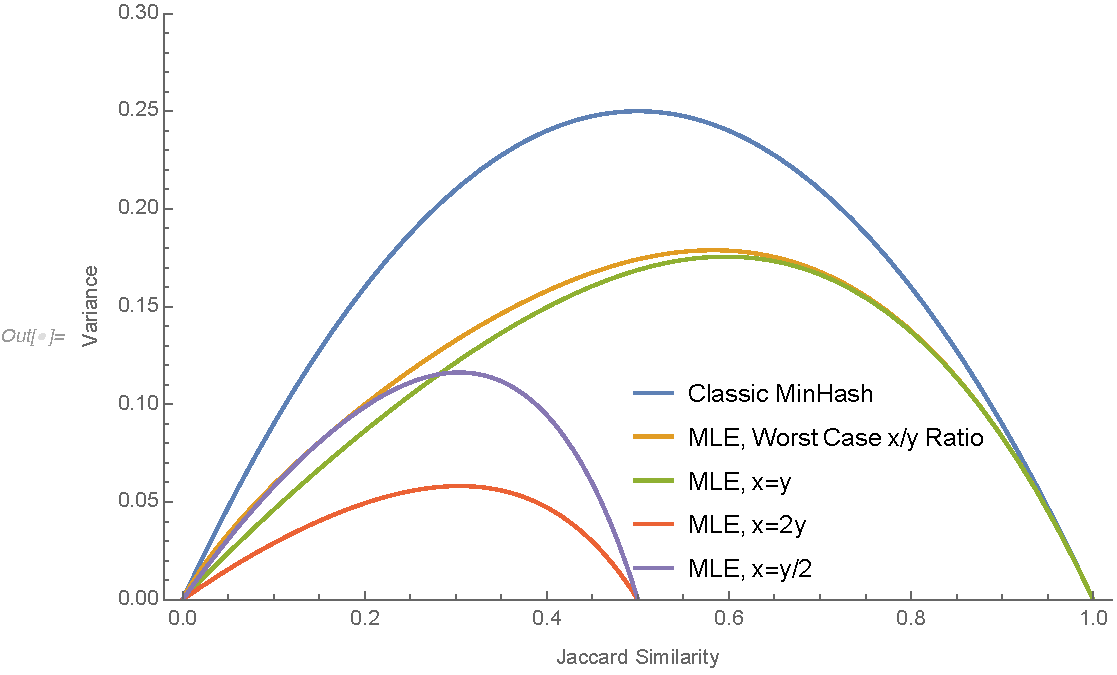
\includegraphics[trim=30 0 0 0,clip,width=\linewidth]{figures/mle_variance2}
\caption{Variance of Maximum Likelihood Estimator based on Fischer Information bound.
For $j$ close to 0 or 1 the worst case MLE bound is asymptotically equal to the Classical bound, whereas for $j\approx 0.21$ has only $\approx 62\%$ of the variance.}
\label{fig:mle_variance}
\end{figure}

We can also compute the global risk of the MLE estimator, which is $0.178847/K$, $28.5\%$ less than the Classical Estimator.

% Nice example to include when we show how to compute the expectations in the MLE bound
% Using
% \begin{align}
%    \frac1{x-v-k+1}\binom{x-k}{v}
%    &=
%    \frac1{x-v-k+1}\binom{x-k}{x-v-k}
%  \\&=
%    \frac1{x-k+1}\binom{x-k+1}{x-v-k+1}
%  \\&=
%    \frac1{x-k+1}\binom{x-k+1}{v}
%  \\&=
%    \frac1{v}\binom{x-k}{v-1}
% \end{align}



\subsection{Effect of approximation}

What can wee still say about the variance of the original estimator given this relaxation?

From http://galton.uchicago.edu/~eichler/stat24600/Handouts/l02.pdf

If the model is incorrectly specified and the data $Y$ are sampled from a true
density $f^*$ then the ML estimate converges to the value $\theta^*$ which minimizes
the Kullback-Leibler information


\subsection{Minner Estimator}

The starting point of this derivation is \cref{eq:deriv1},
to which we apply the approximation $\log(1-\eps) \approx -\eps$,
to get the equation
\[
   \frac{d}{dv}\ell(m;v) \approx
   -\frac{[m\not\in x]}{y-v} 
   -\frac{k}{x-v} 
   +\frac{[m\in x]}{v} 
   +\frac{m-k}{y-x-y+v} 
   = 0.
\]
When observing multiple $m_i's$, let $a=\sum_i [m\not\in x]$ and $b=\sum_i [m\in x]$.
Similarly let $k=\sum_i k_i$ and $m=\sum_i m_i$.
Then we want to solve
\[
   -\frac{a}{y-v} 
   -\frac{k}{x-v} 
   +\frac{b}{v} 
   +\frac{m-k}{y-x-y+v} 
   = 0.
\]
This can be rewritten as a degree three polynomial and solved by standard methods.
However, we would like a simpler estimator still.

In general we assume $u$ is very large, so we'll approximate $\frac{m-k}{u-x-y+v}\approx 0$.
If we further approximate $\frac{a}{y-v}\approx 0$ we get the simple solution $v=\frac{bx}{b+k}$.
This corresponds to the case where $v$ is small compared to $y$.
Alternatively, if we approximate $\frac{k}{x-v}\approx 0$, we get $v=\frac{b y}{a+b}$.
This corresponds to the case where $v$ is small compared to $x$.
From this intuition we propose the following estimator:
\begin{definition}[Minner Estimator]
\[
   T(m) = \min\left\{\frac{bx}{b+k}, \frac{b y}{a+b}\right\}.
   \label{eq:minner}
\]
\end{definition}
The resulting value is clearly always in the acceptable range $[0,\min\{x,y\}]$.

For Jaccard we do $j = v/(|X| + y - v)$

%Another thing: There may still be some cases where there is no solution within the acceptable range.
%I should probably do something about that?

We can improve upon the resulting estimate by Newton's method.
This is a common idea in MLE design. % TODO: Cite somebody?

TODO: I used to have some computations on this estimator as well...
Something like
\[
   E[\frac{bx}{b+k}] = \frac{v}{y} E[\frac{x}{1+k}]
\]
and so on.

\section{Old}


We start from the lower bound side by considering the Cramer Rao bound with $k=1$.
We define a random variable $Z$ to $\inf$ if $m\not\in x$ and $
= \sum_{z\in x\setminus y} [h(z) \le h(m)]$ otherwise.

Note that we can change the distribution of $h$ to be anything monotone without changing the probabilities.
We'll now assume it has exponential distribution.
%(Also note that that $\log 1/h(z)$ has exponential distribution.)
let $h^* = h(m)$, then $h^* = \min_{z\in y}h(z) \sim \text{Exp}(y)$ by stability of minimums.
We define $p=\Pr[h(z)\le h^*] = 1-\exp(-h^*)$.
Conditioning on $h^*$ we see that $Z$ has binomial distribution $B(n,p)$ where $n=|x\setminus y|$.

Back to the lower bound, 
Cramer Rao asks us to define
\[
   I(j) = E_{z,p}\left[\left(\frac{d\ell(z,p;\; j)}{d\ell}\right)^2\right]
\]
where (for $z\not=\inf$)
\begin{align}
   \exp(\ell(z;j))
   &=\Pr[Z=z]
 \\&= \Pr[m\in x]E_{h^*}[\binom{n}{z}p^z(1-p)^{n-z}]
 \\&= \tfrac{v}{y}E_{h^*}[\binom{n}{z} (1-e^{-h^*})^z e^{-h^*(n-z)}]
 \\&= \frac{v}{n+y}\binom{n}{z}\bigg/\binom{n+y-1}{z}
\end{align}
Approximating
\[
   \binom{n}{z}p^z(1-p)^{n-z} \sim \exp(-n D(z/n, p))
\]


Let's assume all the hash values on $x$ are fixed in advance.
Now we pick the values for $y\setminus x$.
We set $m=\argmin_{y_i\in y} h(y_i)$.
We are interested in the probability that $m\in x$ and $m=m^*$ for some element $m^*\in x\cap y$.
We define $h^*=h(m^*)$.

Let $Z$ be the minimum hash value in $y\setminus x$. Then it has distribution $\text{Exp}(|y|-v)$.
We are going to have $m=m^*$ exactly when $Z$ is larger than $h^*$.
(Such that no other value ``wins'' in $y$)
We also need $m$ to be the smallest in $x\cap y$, but that is implied by $m\in x$, since the hash values in $x$ are fixed.
Now $\Pr[Z \ge h^*] = \exp(h^*(|y|-v))$
so the total probability is $\frac{v}{y}\exp(-h^*(|y|-v))$.
This suggest the MLE of $v=-1/h^*$.
That can't be..

Maybe that whole combination argument is wrong.
Surely once we have $\Pr[Z\ge h^*]$ we already have $m\in x$, so we don't actually have that factor $v/y$...

What if I also use information when $m\not\in x$?
I can still compute the hash value of $m$ and compare it to my own hash values...
If $m\not\in x$ we have $Z < h^*$, where again $h^*$ is the smallest hash value in $x\cap y$.
This happens with probability $1-\exp(-h^*(|y|-v))$ which is most likely at $v=0$.
So this suggests a ``bang bang'' estimator, simply dependent on whether $m\in x$.
This is however still different from the normal minhash estimator, which also asks for the value to be smallest in $x$.

